\section{ReMap System Design and Implementation}
ReMap (\autoref{fig:remap_interface}) extends the RePlay contextual search system (Chapter \ref{chapter:replay}) . RePlay enables users to search for learning videos in context while working in software, and it highlights relevant moments in video results based on the user's context and query. While RePlay helps people find results faster, the attentional cost of switching to RePlay discouraged participants from using it more frequently. ReMap lowers the switching cost and cognitive load of help-seeking by introducing three main improvements over RePlay: searching for help using speech, making deictic references in a search query, and navigating video results using speech commands.

\subsection{Searching for Help using Speech}
At any time, the user can search for help by saying the word \textit{``search''} followed by their query (\autoref{fig:remap_interface}a). Much like other speech interfaces (\textit{e.g.,} Siri), ReMap's search field displays the user's query as it is being transcribed. Once the user is finished speaking, ReMap executes a search with the transcribed query. This allows the user to quickly and easily search for help without taking their hands (or mouse) off their current task.

\subsection{Making Deictic References in a Search Query}
Especially with new software, people are often unfamiliar with an application's vocabulary but can point at application elements that are relevant to their goal. 
To alleviate the challenge of remembering application-specific terms, ReMap allows users to deictically reference interface elements and objects while speaking their query. If the user says \textit{``this''} or \textit{``that''} while clicking on a detectable element, ReMap replaces the pronoun with the reference element's name (\autoref{fig:remap_interface}b-c). Like RePlay, ReMap uses \textsc{os} accessibility \textsc{api}s to resolve element names. 
%This \textsc{api} can get the name and description of any element with accessibility labels \cite{Fraser2019}. Many modern applications have labeled menus, buttons, and other interface elements. Some also label canvas elements (such as text boxes, images, and graphics) though many do not. The examples in this demo use Canva (\url{canva.com}) as the primary software. Canva labels most canvas elements and interface buttons.

While ReMap is detecting a speech query, it stores a list of every detectable element clicked. Once the user is finished speaking, ReMap replaces all occurrences of \textit{``this''} and \textit{``that''} with the element names in the order they were clicked before issuing the search query. This means that users need not speak the deictic reference at the exact same time as they click (which people rarely do \cite{Oviatt1999}), they only need to click before they are finished speaking.

\subsection{Navigating Video Results Using Speech Commands}
In addition to dictating search queries, ReMap allows users to navigate video results using speech commands. This was inspired by  Chang \textit{et al.}'s \cite{Chang2019} findings that  people often pause and skip forward or backward when following along with video tutorials so that they can keep pace with the video, skip irrelevant content, or replay sections they need to see again. Chang \textit{et al.} \cite{Chang2019} propose using speech to navigate tutorials for physical tasks so that users do not have to take their hands off the task to navigate videos. Although ReMap is currently intended for digital tasks, not physical, our evaluations of RePlay found that there is still a significant cost to moving one's mouse and attention to a video from a software task, so we expect speech navigation to be similarly helpful for digital tasks. 

ReMap currently supports the following speech commands: \textit{``play''} (plays the first or most-recently played video), \textit{``play \{first, second, third, fourth, fifth\} video''}, \textit{``play \{next, previous, last\}''} (plays the next/previous/last video in the list), \textit{``\{next, previous, repeat\} marker''} (skips to the next or previous timeline marker, or re-starts from the current marker), and \textit{``pause''} / \textit{``stop''} (pauses the currently playing video).


\subsection{Implementation}
\label{sec:remap_implementation}
ReMap is implemented as a MacOS Swift application (\autoref{fig:remap_system}a). Like RePlay, it also has a custom web server that hosts a script for logging usage data and a webpage for displaying YouTube videos. In addition, ReMap's custom server hosts a webpage for detecting speech. ReMap uses socket.io to communicate between the web server and the three client interfaces (the ReMap desktop application, speech webpage, and video player webpages). The web server (\autoref{fig:remap_system}b) is implemented in Node.js. The speech webpage (\autoref{fig:remap_system}c) uses the Web Speech \textsc{api} to detect and transcribe speech, and the video player webpage (\autoref{fig:remap_system}d) uses the YouTube Player \textsc{api} to load and control videos (like RePlay). %ReMap generates a unique anonymous user \textsc{id} for each computer it runs on. 

When launched, ReMap opens the speech webpage in the user's web browser. To display videos, ReMap loads the video player webpage in \texttt{WKWebView} objects. 
Like RePlay, ReMap includes the user's anonymous \textsc{id} as a query parameter for both types of webpages. For video player pages, it also includes that video's index in the result list. The server keeps track of these values for each client page that opens a socket connection, so that it can pass the commands it receives to the appropriate client.

\begin{figure}[b!]
\centering
  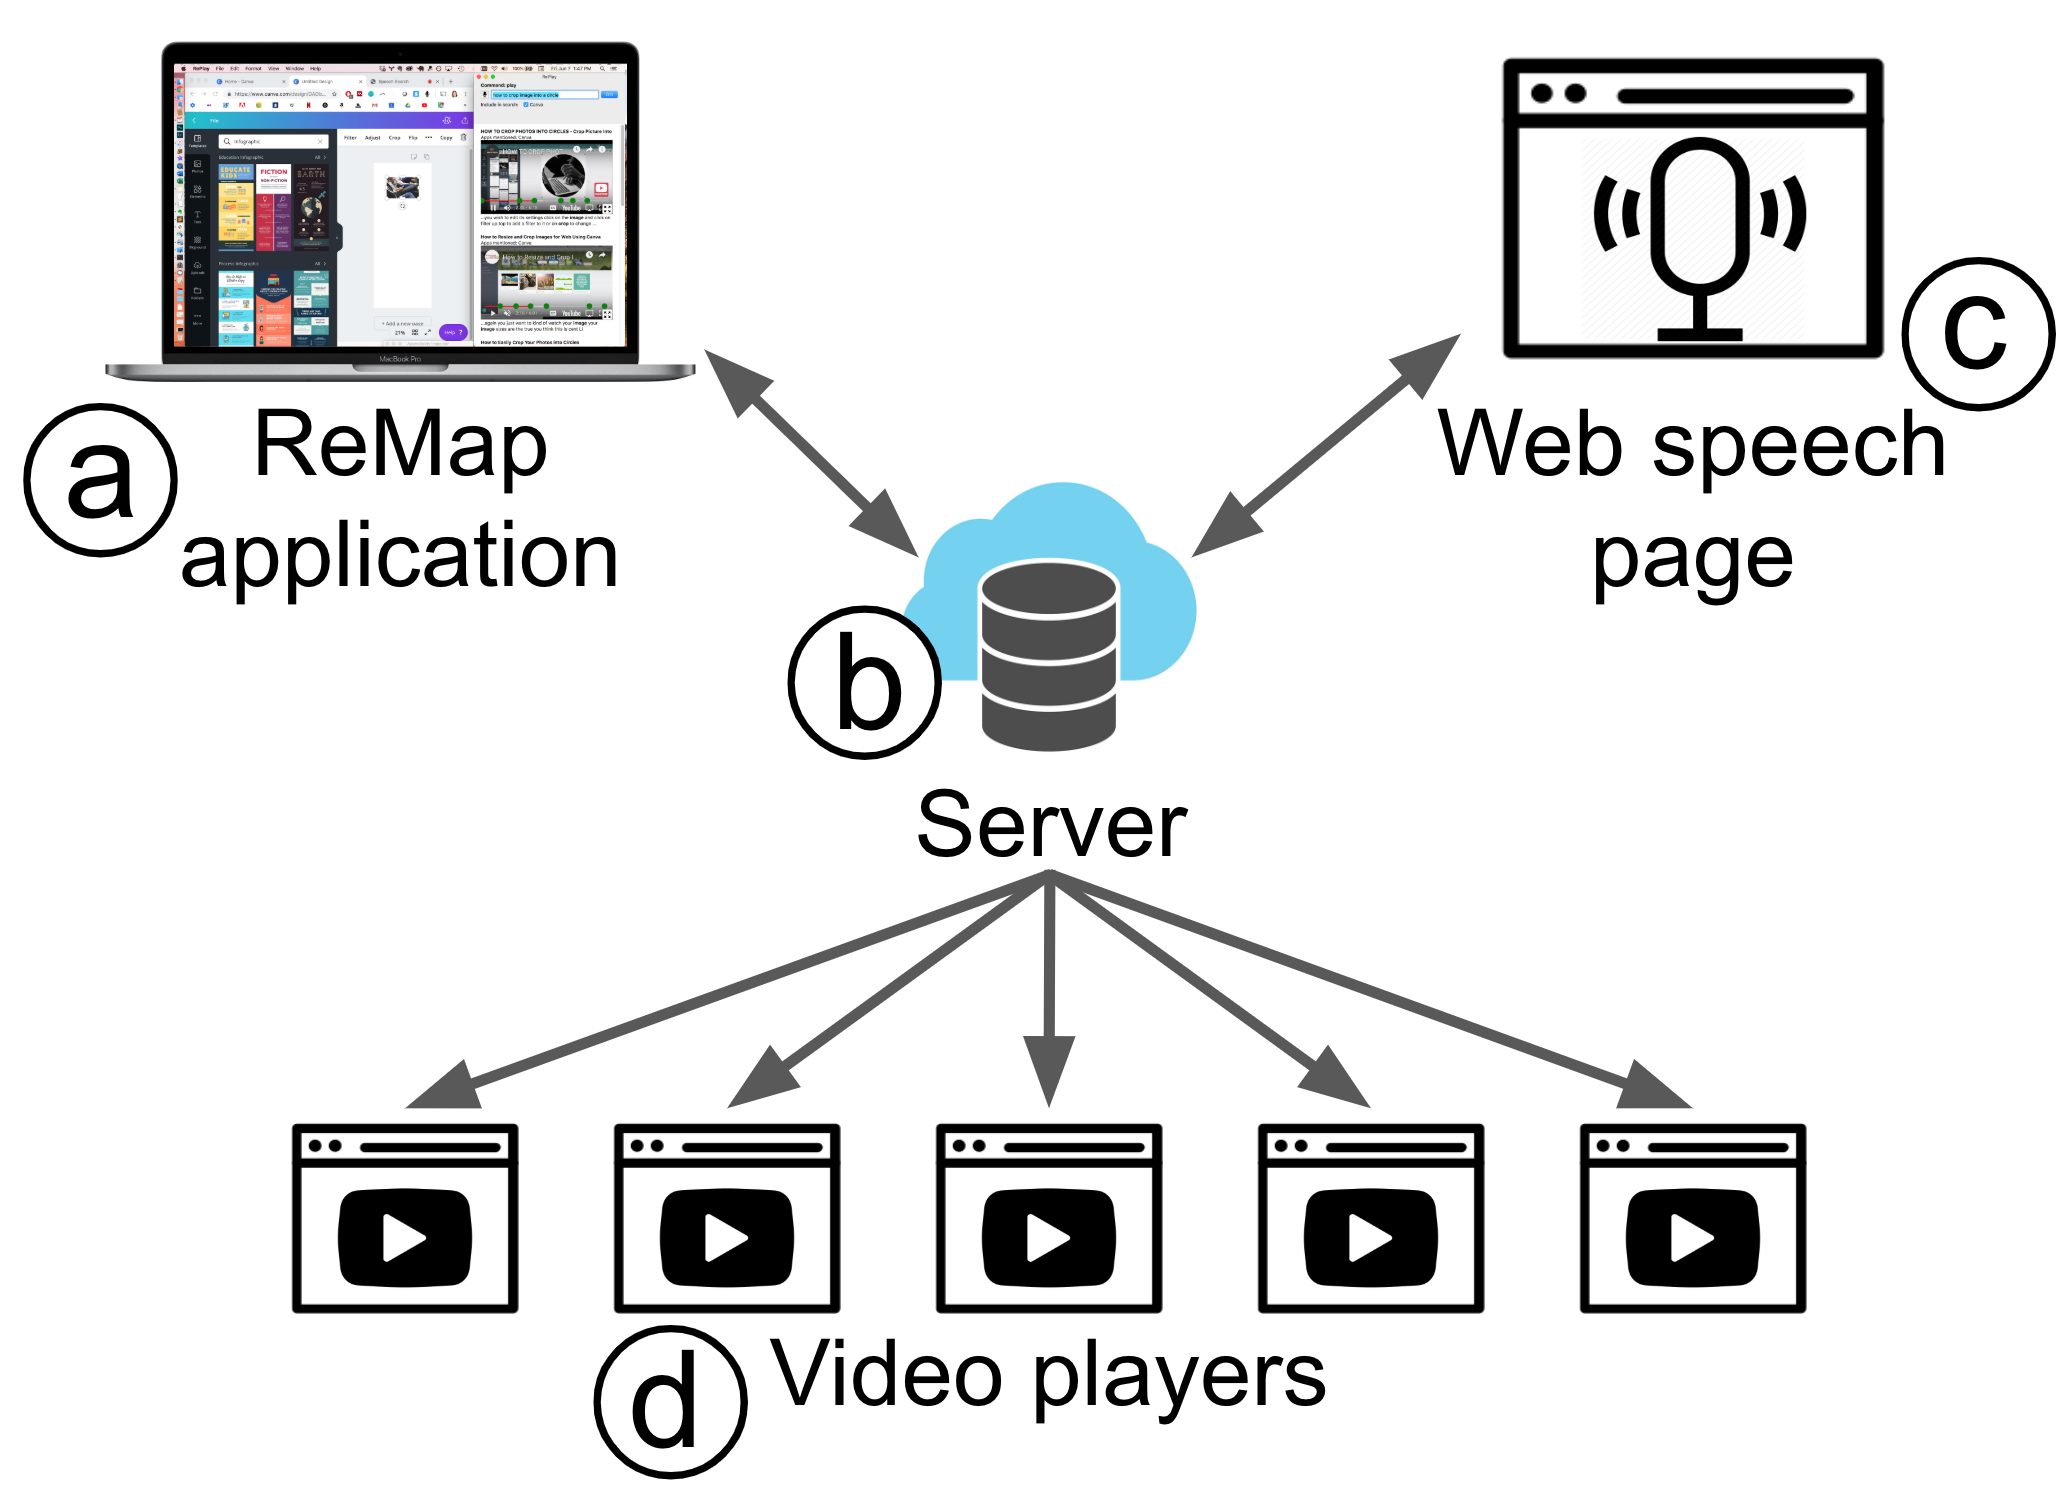
\includegraphics[width=.7\textwidth]{remap/figures/system.png}
  \caption{The ReMap system architecture. a) ReMap is a MacOS application that uses the Accessibility \textsc{api} to detect user context. b) ReMap connects to a custom web server, which hosts c) a webpage for speech recognition and d) a video player webpage embedded in ReMap for each video result.}~\label{fig:remap_system}
\end{figure}

The speech webpage invokes continuous listening using the Web Speech \textsc{api}, so that the user can interact using speech at any time. 
The Web Speech \textsc{api} automatically determines when the user starts and finishes speaking, returning each phrase separately. If a phrase begins with the word \textit{``search''}, the webpage sends the rest of the phrase to the server which sends it to ReMap as a query. As the user continues to speak their query, the speech webpage sends the server the updated phrase every time a new word is detected, so ReMap can display it in real time (\autoref{fig:remap_interface}c).

If the phrase does not start with \textit{``search''} and it matches a video navigation command, the server sends this command to ReMap. ReMap then determines which video index the command applies to, and tells the server which video player client to send the command to. For example, if the third video in ReMap's result list is playing and the user says \textit{``pause''}, the web speech page passes this command to the server which passes it to ReMap. ReMap keeps track of which video is playing, so it then tells the web server to pause the video at index 2. The web server sends a \textit{``pause''} command to the video player client with index 2 that matches the given user \textsc{id}. The video player receives this command and uses JavaScript to pause the YouTube video. If the command is to play a different video than the currently playing video, ReMap also tells the server to pause the currently playing video. 

\subsubsection{Why use a web server?}
Like RePlay, ReMap uses a webpage to display videos because there is no way of incorporating web technologies like JavaScript directly into a MacOS application. It was necessary to build ReMap as a MacOS application so it could have access to the MacOS Accessibility \textsc{api}. 

ReMap uses the Web Speech \textsc{api} to transcribe speech because there is no library for converting arbitrary speech to text in MacOS applications. The only available speech service for MacOS at the time of writing is command recognition (recognizing spoken commands from a pre-defined list). To enable searching by speech, we needed a speech-to-text service that could transcribe arbitrary words. To enable this, we used the Web Speech \textsc{api}, which requires the user to have a browser window open and relies on a steady internet connection for ReMap and the speech client to communicate. We initially used the MacOS command recognition service (\texttt{NSSpeechRecognizer}) for detecting video navigation commands, but found it had greater latency than our Web Speech \textsc{api} approach.

The current implementation works well enough as a research prototype; it can detect and transcribe speech with no noticeable delay on an average internet connection. The speech webpage can be minimized or hidden by the user, and it only asks the user to grant access to the microphone the first time it is opened; all subsequent uses grant access automatically. However, to support a large number of users and avoid needing to open a webpage, a commercial system could instead implement custom in-house speech detection. Further, we hope that in the future, an architecture that allows both web technology and accessibility \textsc{api} access might eliminate the need for a web server entirely, thus simplifying ReMap's implementation substantially. 






